% !TeX program = xelatex
\begin{filecontents*}{audit-references.bib}
@book{liu2013,
  author = {刘海洋},
  title = {{LaTeX} 入门},
  address = {北京},
  publisher = {电子工业出版社},
  year = {2013}
}
@online{amsmathGuide,
  author = {{American Mathematical Society} and {The LaTeX Project}},
  title = {User's Guide for the {amsmath} Package},
  year = {2020},
  url = {https://tug.ctan.org/macros/latex/required/amsmath/amsldoc.pdf},
  urldate = {2026-11-04}
}
\end{filecontents*}
\documentclass[UTF8,11pt,a4paper,twoside,openany,fontset=none,linespread=1]{ctexbook}
\usepackage{fvextra,array,needspace,gbt7714}
\bibliographystyle{gbt7714-numerical}
\defaultCJKfontfeatures{} % 避免请求字体未提供的 CJK 脚本特性
\newif\ifwinfonts
\IfFontExistsTF{SimSun}{\IfFontExistsTF{SimHei}{%
  \IfFontExistsTF{KaiTi}{\winfontstrue}{} }{} }{}
\ifwinfonts
  \setCJKmainfont[BoldFont=SimHei,ItalicFont=KaiTi]{SimSun}
  \setCJKsansfont[BoldFont=SimHei]{SimHei}
  \setCJKmonofont{SimSun}
\else
\setCJKmainfont[BoldFont=FandolSong-Bold,
  ItalicFont=FandolKai-Regular]{FandolSong-Regular}
\setCJKsansfont[BoldFont=FandolHei-Bold]{FandolHei-Regular}
\setCJKmonofont{FandolFang-Regular}
\fi

% ===== 1. 页面尺寸、边距与页眉页脚 =====
\usepackage{geometry}
\geometry{
  a4paper,
  inner=26mm,outer=23mm,    % 内侧靠书脊，多留 3 mm；偶数页自动镜像
  top=25mm,bottom=25mm,
  includeheadfoot,         % 上下边距按“含页眉页脚的整体区域”计算
  headheight=16pt,         % 为页眉内容预留高度
  headsep=6mm,footskip=10mm
}
% 不再另加 bindingoffset：这套内边距已考虑日常薄册装订。

% ===== 2. 行距与段落间距 =====
\usepackage{setspace}
\setstretch{1.35}          % 标准基线距离的 1.35 倍，不是字号的 1.35 倍
\setlength{\parindent}{2\ccwd} % 首行缩进两个汉字
\setlength{\parskip}{3pt plus 1pt minus 1pt}
\raggedbottom             % 允许页底留白，避免为了齐底过度拉伸段落间距

% ===== 3. 数学环境与图表 =====
\usepackage{amsmath,amssymb,mathtools,bm}
\usepackage{graphicx,booktabs,tabularx,longtable}
\usepackage{pgfplots}
\pgfplotsset{compat=1.18}
\usepackage{enumitem}
\setlist{leftmargin=2\ccwd,itemsep=3pt,topsep=6pt}
\renewcommand{\arraystretch}{1.2} % 适当增加表格行高
\setlength{\jot}{5pt}           % 增加多行公式的行间距
\numberwithin{equation}{chapter}
\newcommand{\dd}{\mathop{}\!\mathrm{d}} % 微分符号采用直立体，并调整前置间距
\newcommand{\R}{\mathbb{R}}
\newcommand{\vect}[1]{\bm{#1}}

% ===== 4. 配色与知识卡片 =====
\usepackage{xcolor}
\definecolor{Ink}{HTML}{19364A}
\definecolor{Teal}{HTML}{227C81}
\definecolor{Gold}{HTML}{A87830}
\definecolor{Rust}{HTML}{9B483A}
\definecolor{CoverTeal}{HTML}{20ADAA}
\usepackage{tikz}
\usepackage[most]{tcolorbox}
\tcbset{
  enhanced,breakable,boxrule=0.45pt,arc=1mm,
  left=3mm,right=3mm,top=2mm,bottom=2mm,
  before skip=10pt,after skip=10pt,lines before break=3,
  colback=Teal!3!white,colframe=Teal,fonttitle=\bfseries
}
\newtcolorbox{conceptbox}[1]{title={概念：#1},colframe=Ink,colback=Ink!3!white}
\newtcolorbox{methodbox}[1]{title={方法卡：#1}}
\newtcolorbox{pitfallbox}{title=我踩过的坑,
  colframe=Rust,colback=Rust!3!white}
\newtcbtheorem[number within=chapter]{notetheorem}{定理}
  {colframe=Ink,colback=Ink!3!white}{thm}

% ===== 5. 标题层级与页眉 =====
\ctexset{
  chapter={format=\huge\bfseries\color{Ink},
    beforeskip=8pt,afterskip=20pt},
  section={format=\Large\bfseries\color{Teal},
    beforeskip=18pt,afterskip=9pt},
  subsection={format=\large\bfseries\color{Ink},
    beforeskip=12pt,afterskip=6pt}
}
\setcounter{tocdepth}{2}
\setcounter{secnumdepth}{2}
\let\cleardoublepage\clearpage % 这份学习册不强制补偶数空白页
\usepackage{fancyhdr}
\pagestyle{fancy}
\fancyhf{}
\fancyhead[LE,RO]{\small\color{Ink}\thepage}
\fancyhead[LO]{\small\nouppercase{\leftmark}}
\fancyhead[RE]{\small\color{Ink}从笔记到论文}
\renewcommand{\chaptermark}[1]{\markboth{第\thechapter 章\quad #1}{}}
\renewcommand{\headrulewidth}{0.4pt}
\fancypagestyle{plain}{% 章首页的页码放在页脚
  \fancyhf{}\fancyfoot[C]{\small\thepage}
  \renewcommand{\headrulewidth}{0pt}
}

% ===== 6. 封面：图片与文字分别排版 =====
% 图片可选：把 cover_banner.png 放在 main.tex 同目录即可。
% 没有图片时使用数学表达式封面，仍可独立编译。
\newcommand{\makecover}{%
  \begin{titlepage}\thispagestyle{empty}
  \begin{tikzpicture}[remember picture,overlay]
    \begin{scope}
      \clip (current page.north west) rectangle
        ([yshift=-76mm]current page.north east);
      \fill[Ink!5] (current page.north west) rectangle
        ([yshift=-76mm]current page.north east);
      \IfFileExists{cover_banner.png}{%
        \node[inner sep=0pt] at ([yshift=-38mm]current page.north)
          {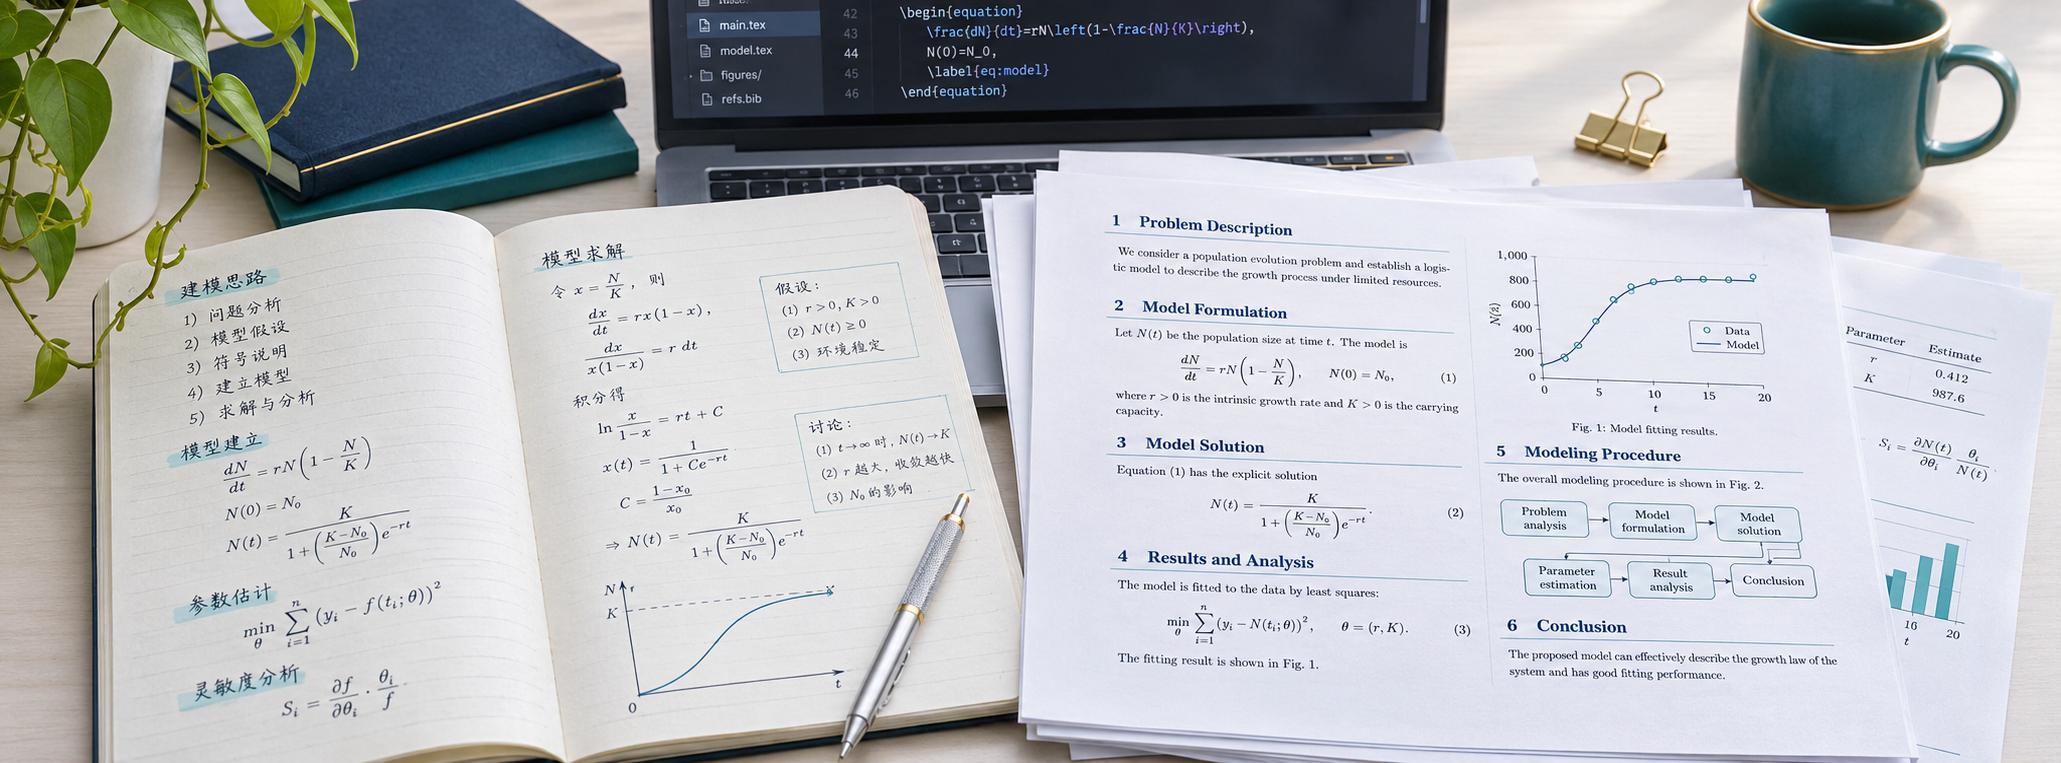
\includegraphics[width=\paperwidth]{cover_banner.png}};
      }{%
        \node[text=Teal] at ([yshift=-38mm]current page.north)
          {\fontsize{32}{40}\selectfont
           $\displaystyle\int_a^b f(x)\,\dd x\qquad\bm{A}\bm{x}=\bm{b}$};
      }
    \end{scope}
    \fill[CoverTeal] ([yshift=-76mm]current page.north west)
      rectangle ([yshift=-86mm]current page.north east);
    \node[anchor=north west,text=Ink,inner sep=0pt] at
      ([xshift=20mm,yshift=-108mm]current page.north west)
      {\fontsize{32}{40}\selectfont\sffamily\bfseries 从笔记到论文};
    \node[anchor=north west,text=Ink,inner sep=0pt] at
      ([xshift=20mm,yshift=-131mm]current page.north west)
      {\fontsize{21}{29}\selectfont\bfseries\LaTeX{} 数学排版实战指南};
    \node[anchor=north west,text=Teal,inner sep=0pt] at
      ([xshift=20mm,yshift=-153mm]current page.north west)
      {\large 数学复习笔记\quad /\quad 数学建模写作};
    \node[anchor=north west,text=black!60,align=left,inner sep=0pt] at
      ([xshift=20mm,yshift=-184mm]current page.north west)
      {雪落长安无声\\[5mm]版本：修订版\\[5mm]日期：2026.11.04};
    \draw[Gold,line width=0.7pt]
      ([xshift=20mm,yshift=45mm]current page.south west) --
      ([xshift=-20mm,yshift=45mm]current page.south east);
    \node[text=Ink] at ([yshift=32mm]current page.south)
      {让公式有呼吸，让论证有秩序。};
  \end{tikzpicture}
  \null\end{titlepage}
}

% ===== 7. PDF 链接、书签与元数据 =====
% 常规宏包先加载，hyperref 靠后；其他宏包另有顺序要求时按其说明处理。
\newif\ifprintversion
\printversionfalse          % 纸质版改成 true；这里选屏幕阅读版
\usepackage[unicode]{hyperref}
\hypersetup{
  pdftitle={从笔记到论文：LaTeX 数学排版实战指南},
  pdfauthor={雪落长安无声},
  pdfsubject={数学笔记与数学建模写作},
  bookmarksnumbered=true,bookmarksopen=true,bookmarksopenlevel=1,
  linktoc=all,
  colorlinks=true,linkcolor=Teal,citecolor=Teal,urlcolor=Teal
}
\ifprintversion
  \hypersetup{hidelinks}    % 隐藏链接颜色和边框，保留点击功能
\fi

% ===== 正文内容 =====

\usepackage{attachfile2}
\newcommand{\E}{\mathbb{E}}
\DeclareMathOperator{\Cov}{Cov}
\fvset{fontsize=\footnotesize,breaklines=true,breakanywhere=true,
  numbers=left,numbersep=5pt,xleftmargin=5mm,baselinestretch=1.1,
  frame=leftline,rulecolor=\color{Teal!35}}
\newcommand{\sourceattachment}[1]{%
  \par\smallskip\noindent{\small\color{Teal}%
    \edef\attachsource{\noexpand\attachfile
      [mimetype=text/plain,color=0.13 0.49 0.51]{\detokenize{#1}}}%
    \attachsource
    \quad 原始源码 \nolinkurl{#1}}\par\smallskip
}
\newcommand{\examplecode}[1]{%
  \par\medskip\Needspace{6\baselineskip}%
  \noindent{\small\bfseries 完整可编译示例}\par\smallskip
  \sourceattachment{#1}%
  \begingroup\setstretch{1}\VerbatimInput{#1}\endgroup
}
\newcommand{\examplepreview}[2][.94\linewidth]{%
  \par\medskip\noindent
  \begin{minipage}{\linewidth}
    {\small\bfseries\color{Ink}编译效果}\par\smallskip
    \centering\includegraphics[width=#1,height=.56\textheight,keepaspectratio]{#2}
  \end{minipage}\par\medskip
}
\begin{document}
\hypersetup{pageanchor=false}\makecover\hypersetup{pageanchor=true}
\frontmatter
\chapter{写在前面}
我把写数学笔记和数模论文时常用的排版方法放进了这本书。前六章从一套导言区起步，
逐步加进公式、图表、知识框和交叉引用。第六章把这些零件装进同一份复习笔记，
最后两章再转到竞赛论文的摘要、算法和文献。

读到想动手的地方，可以从随书的 \texttt{.tex} 文件开始。第二、四、六、八章各有一份包含正文的独立文档。
代码清单旁标有源文件路径和附件图标。可以用支持附件的 PDF 阅读器保存原始源码，也可以从随书压缩包取用对应的文件。书中的行号和折行用于阅读定位。
本文档使用 XeLaTeX，目录与交叉引用通常要编译两遍，参考文献按第八章的四步流程处理。
\tableofcontents
\mainmatter
\chapter{留白、行距与导言区}

我刚开始写数学笔记时，总觉得公式能编译出来就算完成。等到复习，才发现有些页根本不想看：段落挤，分式挤，连公式编号也挤。我开始认真调整页边距和行距，后来把这些设置固定下来，写新章节时便不用从头折腾。

这份模板沿用高数、线代、概率论三套笔记的深蓝与青绿配色。定理、方法和计算提醒各有固定样式；公式与图表自动编号，PDF 中的引用可以点击。封面的图片和文字分开处理，改书名时不用重做整张图。

导言区已经加载第二至四章示例所需的数学、图表宏包，也定义了概念框和向量命令。迁移这些示例时，取文档起止命令之间的内容，按书中的章节层级调整标题。算法、子图和文献示例用到的额外宏包，则按各章的说明加入导言区。

这是学习用书和复习笔记的模板。参赛稿有自己的格式要求，第七章会单独处理摘要页。

\section{先编译一份完整文档}

把代码存为 main.tex，编码设为 UTF-8，选择 XeLaTeX，连续编译两遍。默认使用已有的中文字体；缺少 Windows 字体时会回退到 Fandol。需要的宏包应已安装，不用开启 shell escape。

封面图不是必需文件。有图就把它命名为 cover\_banner.png，放在 main.tex 旁边；没有图也能编译。我建议你先确认正文、目录和引用都正常，再换自己的封面。

本章末尾给出了\hyperref[sec:golden-template-source]{完整模板源码}。本书封面使用同一套设计，下图展示示例的正文页。
\examplepreview{previews/ch01_01_example-p3.png}

\section{geometry：把页边距算清楚}

这套参数采用 A4 纸，内侧 26 mm，外侧 23 mm。我把靠书脊的一侧多留了 3 mm，方便翻页和薄册装订。双面模式下，奇数页与偶数页会自动交换内外侧，页眉也随之镜像。

{\centering\begin{tabular}{@{}>{\raggedright\arraybackslash}p{.21\linewidth}>{\raggedright\arraybackslash}p{.29\linewidth}>{\raggedright\arraybackslash}p{.43\linewidth}@{}}
\toprule
参数 & 取值 & 含义 \\
\midrule
inner / outer & 26 / 23 mm & 靠书脊与纸张外侧的边距 \\
top / bottom & 各 25 mm & 含页眉页脚区域到纸张上下边缘的距离 \\
includeheadfoot & 开启 & 计算总版心时计入页眉、页眉间隔与页脚距离 \\
headheight & 16 pt & 页眉预留高度 \\
headsep & 6 mm & 页眉与正文之间的距离 \\
footskip & 10 mm & 正文区域底边到页脚基线的距离 \\
\bottomrule
\end{tabular}\par}

includeheadfoot 最容易被忽略。开启后，上下 25 mm 并不等于正文离纸边各 25 mm。A4 的高度是 297 mm，扣掉上下边距得到 247 mm，这部分还要容纳页眉与页脚所需的空间，所以真正的正文高度会更小。

正文宽度是 210 mm 减去 26 mm 和 23 mm，等于 161 mm。碰到特别长的公式，我会先尝试按推导步骤拆行。

做单面活页笔记时，可以把 twoside 改成 oneside，并同步调整页眉位置。厚册胶装则应根据纸张、页数和装订方式重新评估内边距。这组数值是我的起点，不是通用的“黄金比例”；模板也没有另外叠加 bindingoffset，免得装订空间加了两次。

\section{setspace：行距、段距分开调}

中文笔画密，公式又有分式和上下标，行距太小会明显影响阅读。我把 ctex 的初始倍率设为 1，再用 setspace 统一设成 1.35，免得几处行距命令相互覆盖。

\textbf{1.35 乘的是当前字号的标准基线距离。} 这套 11 pt 文档的标准基线为 13.6 pt，调整后约为 18.36 pt。遇到较高的行内公式，实际基线距离还可能增加。

我建议你拿两页真实内容试排，别只看一行测试文字。文字多时可以稍收紧，分式和推导多时再适当放宽。

段距单独设置为约 3 pt，并保留两字首行缩进；表格行高交给 arraystretch，多行公式的额外间隔交给 jot。不要指望一个行距倍率把所有间隔都调好。

我还开启了 raggedbottom。内容不足一页时，允许页底留白，尽量不为了齐底而把段落间距拉大。这里的留白由版式处理，不靠反复敲空行来凑。

\section{hyperref：引用、书签与文件信息}

当笔记请读者回看式~(7.23) 时，超链接可以省去来回翻页。hyperref 能让读者点击目录或公式编号直接跳转，也能打开正文里的网址。

colorlinks 用文字颜色标识链接；linkcolor 管内部引用，urlcolor 管网址，citecolor 管文献引用。我把三者统一为深青绿。本例尚未接入文献数据库，citecolor 先预留。

bookmarksnumbered 为侧边栏书签显示编号，bookmarksopen 与 bookmarksopenlevel 控制默认展开方式。linktoc 设为 all，目录标题和页码就都能点击。侧边栏书签与正文目录各自独立，阅读器还可能记住自己的展开偏好。

pdftitle、pdfauthor、pdfsubject 写入 PDF 元数据，封面文字仍需单独排版。做匿名稿时，署名、页眉和元数据都要检查，只删封面上的姓名还不够。

屏幕版保留青色链接。打印时把开关改为 true，hidelinks 会隐藏颜色和边框，点击功能还在。这个开关只改链接外观，不会自动把学习模板变成竞赛稿。

我把 hyperref 放在常规数学、图表和版式宏包后面。它不必永远是最后一个宏包；例如以后加入 cleveref，就应按相应说明处理加载顺序。

\section{这套样式怎样使用}

定理框放条件与结论，方法卡放可执行步骤，踩坑框只提醒确实容易出错的地方。它们都允许跨页，不过长篇推导仍适合用普通正文。每段都装进彩框，层次反而不清楚。

我保留了三部曲中的配色和卡片结构，同时加入公式引用、图表编号和三线表。示例先交代适用条件，再给公式和解释。表中的误差数值只用于演示版式，不是实验结果。

封面命令在导言区定义，在正文开始后调用。第一次改模板，先替换书名和内容；熟悉之后再调 TikZ 坐标。我不建议你同时修改十几处设置，编译出了问题很难定位。

\section{我会先检查这些地方}

编译失败，先看编译器与编码。本书统一使用 XeLaTeX 和 UTF-8。首行的编辑器提示不一定会替你切换实际编译器，仍要检查下拉菜单。中文并非只能用 XeLaTeX 排，但整本书沿用一条编译路线，排错会省事得多。

目录或引用出现问号，先再编译一次；还没解决，再查标签拼写与重复定义。导言区也别整段叠加：原模板已加载的宏包，不用为了“更保险”再加载一遍。旧资料中的 pdftex 驱动选项尤其不能机械搬到 XeLaTeX 配置里。

找不到图片，就核对文件名、扩展名和路径。把 JPG 的后缀改成 PNG，不会改变它的文件格式。

排完一定看 PDF。长公式越界就拆行，别把字号缩成蚂蚁开会。正式交稿前，再按当届要求检查匿名信息、边距、摘要与附录。

\section*{参考资料与配置核对}

版式参考数学三部曲笔记，参数含义结合中文入门资料与宏包说明核对：

\begin{itemize}
\item \href{https://ctan.org/pkg/geometry}{geometry}：页面尺寸与边距。
\item \href{https://ctan.org/pkg/setspace}{setspace}：行距控制。
\item \href{https://ctan.org/pkg/hyperref}{hyperref}：链接、书签与元数据。
\item \href{https://ctan.org/pkg/ctex}{CTeX}：中文文档类、字体与初始行距。
\end{itemize}

\section*{完整模板源码}\label{sec:golden-template-source}
\sourceattachment{examples/ch01/01_example.tex}
\VerbatimInput[baselinestretch=1.04]{examples/ch01/01_example.tex}

\chapter{数学公式与符号的极简美学}

\section{行内、行间与括号}
我把变量和短条件放在句子里，例如 \(x>0\)、\(f(x)=\ln x\)。
需要停下来读的结论则单独成行：
\[
  \int_0^1x^2\,\mathrm{d}x=\frac13.
\]
需要引用时，使用自动编号：
\begin{equation}\label{eq:two:ftc}
  \int_a^b f(x)\,\mathrm{d}x=F(b)-F(a).
\end{equation}
这里假设 \(f\) 在 \([a,b]\) 上连续，\(F\) 在 \([a,b]\) 上连续，
并且在 \((a,b)\) 内满足 \(F'=f\)。
式~\eqref{eq:two:ftc} 的引用通常要编译两遍才稳定。

在源码里，\verb|\(| 与 \verb|\)| 把短公式留在句子里，
\verb|\[| 与 \verb|\]| 让公式另起一行且不编号。
这些定界符本身不印出来。要在公式里印出集合花括号，用 \verb|\{| 和 \verb|\}|。
\[
  (a+b),\quad [a,b],\quad \{x\in\mathbb R\mid x>0\},
  \quad \left(\frac{a+b}{c}\right)^2,
  \quad \left.\frac{x^3}{3}\right|_0^1.
\]
\verb|\left| 与 \verb|\right| 必须配对。单边竖线用点补上不可见的一侧。
别把一对自动伸缩括号直接拆到 align 的两行。

\section{align：把等号对齐}
我用高数笔记中的分部积分题演示连续推导：
\begin{align}
  \int x\mathrm{e}^x\,\mathrm{d}x
    &=x\mathrm{e}^x-\int\mathrm{e}^x\,\mathrm{d}x\notag\\
    &=x\mathrm{e}^x-\mathrm{e}^x+C\notag\\
    &=(x-1)\mathrm{e}^x+C.
\end{align}
\verb|&| 放在等号前，两个反斜杠结束一行。\verb|\notag| 取消该行编号。
align 自己就是行间环境，不要再套一层数学定界符。
整组只要一个编号时，可以这样写：
\begin{equation}
  \begin{aligned}
    (x+1)^2&=x^2+2x+1,\\
    (x-1)^2&=x^2-2x+1.
  \end{aligned}
\end{equation}
aligned 是内部结构，外层 equation 负责整组编号。

\section{矩阵与分段函数}
线代中的方程组可以写成
\[
  \begin{pmatrix}1&1\\2&-1\end{pmatrix}
  \begin{pmatrix}x\\y\end{pmatrix}
  =\begin{pmatrix}3\\0\end{pmatrix},\qquad
  \begin{pmatrix}x\\y\end{pmatrix}=\begin{pmatrix}1\\2\end{pmatrix}.
\]
pmatrix 自带圆括号，\verb|&| 分列，两个反斜杠换行。
先数每行的列数，再怀疑编译器，顺序别反了。

cases 的左列写结果，右列写条件：
\[
  g(x)=\begin{cases}-x,&x<0,\\x,&x\geq0.\end{cases}
\]
概率论里的正部截断也可以直接排成分段形式。
设 \(X\sim U(-1,1)\)，\(Y=\max\{X,0\}\)，则
\[
  F_Y(t)=\begin{cases}
    0,&t<0,\\[3pt]
    \dfrac{t+1}{2},&0\leq t<1,\\[3pt]
    1,&t\geq1.
  \end{cases}
\]
零点属于中间一段，\(F_Y(0)=1/2\)，不能把这个概率跳跃删掉。

\section{向量与希腊字母}
在这套数学字体下，mathbf 常用于粗直立拉丁字母，bm 可处理粗斜体与希腊字母：
\[
  x,\quad\mathbf{x},\quad\bm{x},\qquad
  \alpha,\quad\bm{\alpha},\qquad\mathbf{A}\bm{x}=\bm{b}.
\]
我只加粗向量主体，例如 \(\bm{x}_i\)，下标通常保持普通字重。
函数名使用运算符命令，例如 \(\sin x\)、\(\ln x\)。
少一个反斜杠，有时不报错，只是把函数排成几个散步的字母。

\section{高频符号速查}
中列给出数学模式内的输入，右列显示效果。
\begin{center}
\begin{tabular}{lll}
\toprule
用途 & 输入 & 效果 \\
\midrule
分式 & \verb|\frac{a}{b}| & \(\frac ab\) \\
根式 & \verb|\sqrt{x}| & \(\sqrt{x}\) \\
导数 & \verb|f'(x)| & \(f'(x)\) \\
偏导 & \verb|\frac{\partial f}{\partial x}| & \(\frac{\partial f}{\partial x}\) \\
积分 & \verb|\int_a^b f(x)\,\mathrm{d}x| & \(\int_a^b f(x)\,\mathrm{d}x\) \\
极限 & \verb|\lim_{x\to0}f(x)| & \(\lim_{x\to0}f(x)\) \\
求和 & \verb|\sum_{i=1}^n x_i| & \(\sum_{i=1}^n x_i\) \\
\bottomrule
\end{tabular}
\end{center}
\begin{center}
\begin{tabular}{lll}
\toprule
用途 & 输入 & 效果 \\
\midrule
希腊字母 & \verb|\alpha,\beta,\gamma| & \(\alpha,\beta,\gamma\) \\
常用参数 & \verb|\theta,\lambda,\sigma| & \(\theta,\lambda,\sigma\) \\
大小写 & \verb|\delta,\Delta,\Omega| & \(\delta,\Delta,\Omega\) \\
数集 & \verb|\mathbb{R},\mathbb{N}| & \(\mathbb{R},\mathbb{N}\) \\
属于 & \verb|\in,\notin| & \(\in,\notin\) \\
包含 & \verb|\subseteq,\subsetneq| & \(\subseteq,\subsetneq\) \\
交并 & \verb|A\cap B,A\cup B| & \(A\cap B,A\cup B\) \\
空集 & \verb|\varnothing| & \(\varnothing\) \\
\bottomrule
\end{tabular}
\end{center}
符号只记得形状时，我会用 \href{https://detexify.kirelabs.org/}{Detexify}
画出来查命令，再检查是否需要额外宏包。

\section*{本章完整源码}
\sourceattachment{clean_chapters/ch02.tex}
\VerbatimInput{clean_chapters/ch02.tex}

\chapter{图片、三维曲面与结果表}

我做建模图表时，会先决定读者要比较什么：预测和观测的差异，参数变化带来的误差，还是几种方法的结果。图题、坐标与单位交代清楚，再考虑颜色。只把图放进去，离“结果讲清楚”还差一步。

\section{插入 MATLAB 或 Python 导出的数据图}

我在随书文件中放了一张 Python 导出的示例图，使用六组明确标为演示的数据。它不是实验结论。换成自己的图时，保留坐标名称、单位和图例，不要把软件窗口边框一起截进来。

代码查找同目录的 model\_comparison.png。如果文件尚未准备好，会显示缺图提示，不会因为缺图而中断编译。

\begin{tcolorbox}[colback=Teal!4,colframe=Teal,boxrule=.7pt,arc=1mm,fontupper=\small\bfseries]\textbf{【特别说明】本节使用独立小样。编号和交叉引用通常需要编译两遍。搬回第一章的 ctexbook 模板时，复制文档起止命令之间的正文。}\end{tcolorbox}

\examplecode{examples/ch03/01_image.tex}
\examplepreview{previews/ch03_01_image-p1.png}

includegraphics 负责读入文件，figure 负责浮动位置、图题和编号。这里把图片宽度设为当前行宽的 82\%，不另设高度，原有比例就能保留。若同时指定宽高，应考虑 keepaspectratio，避免拉伸。

caption 建立图号，label 放在它后面。新图片换进来，图题也要改。不要只把“示例图”三个字换成“实验结果”，数据来源与验证过程还得由自己完成。

\section{图片为什么又跑到下一页}

剩下四厘米，要塞一张十厘米高的图，谁来都放不下。图片总是“不听话”，往往只是当前页面没有足够空间。

htbp 是允许位置的集合：h 靠近源码位置，t 页顶，b 页底，p 单独的浮动页。它不是坐标，也不保证严格按字母顺序尝试。排版器还要处理前面没有排出的浮动体。

我先检查尺寸和图表积压，再考虑限制位置。把所有图都强制固定，可能只换来一块大空白。图片里的长说明尽量移到图题或正文，也能减少图片本身的高度。

\section{pgfplots：画一个误差曲面}

我用一个二参数目标函数示意参数搜索：横纵轴是两个待估参数，高度是目标函数值，颜色也表示同一个值。曲面能看出整体形状；若主要任务是读取平面位置，改成热力图通常更方便。

\begin{tcolorbox}[colback=Teal!4,colframe=Teal,boxrule=.7pt,arc=1mm,fontupper=\small\bfseries]\textbf{【特别说明】本节使用独立小样。编号和交叉引用通常需要编译两遍。搬回第一章的 ctexbook 模板时，复制文档起止命令之间的正文。}\end{tcolorbox}

\examplecode{examples/ch03/02_plot.tex}
\examplepreview{previews/ch03_02_plot-p1.png}

addplot3 的 surf 生成曲面，domain 和 y domain 决定两个参数的取值范围。samples 与 samples y 控制两个方向的采样数量。shader=interp 对网格间的颜色进行插值，图会更平滑；增加采样也会增加编译开销，不必一开始就把数量调得很大。

view 的两个角度控制观察方向与仰角。示例从方位角 55 度、仰角 30 度观察；想看俯视效果，可试 view=\{0\}\{90\}。视角只改变看法，不改变函数值。曲面挡住关键区域时，我会先换角度，而不是马上换模型。

colormap/viridis 选择顺序色图，colorbar 显示颜色与数值的对应关系。这里高度和颜色都代表 J；如果颜色另有含义，必须明确说明。不同方案之间比较时，还应统一颜色范围，不能一张图深色代表 1，另一张图却代表 100。

示例的理论最小值由两个平方项直接算出。颜色和网格取自有限采样，不能用来精确读出极小值。实际建模可以把计算结果整理成坐标表再绘图，或在 Python、MATLAB 中处理后导出。\href{https://tikz.dev/pgfplots/reference-3dplots}{pgfplots 三维绘图文档}

\section{用三线表比较方法}

同一组演示数据，先排普通网格表，再用 booktabs 去掉不必要的边线。

\begin{tcolorbox}[colback=Teal!4,colframe=Teal,boxrule=.7pt,arc=1mm,fontupper=\small\bfseries]\textbf{【特别说明】本节使用独立小样。编号和交叉引用通常需要编译两遍。搬回第一章的 ctexbook 模板时，复制文档起止命令之间的正文。}\end{tcolorbox}

\examplecode{examples/ch03/03_tables.tex}
\examplepreview{previews/ch03_03_tables-p1.png}

tabular 定义行列，table 提供浮动位置、标题与编号。l、c、r 分别表示左、中、右对齐；\& 分列，两个反斜杠换行。每行元素数必须与列格式一致。

三线表用 \verb|\toprule|、\verb|\midrule| 和 \verb|\bottomrule| 划出表头与数据区，通常省去竖线和逐行横线。我会先统一同一指标的单位和小数位数，再调整表格线。

需要精确对齐小数点时，再考虑 siunitx。表题写清比较对象；统计量与单位也要能在表内或附近找到，不让读者回翻几页猜含义。

\chapter{自定义环境与常用命令}

\section{列表该不该编号}
并列的材料用 itemize，有先后顺序的步骤用 enumerate。
\begin{itemize}
  \item 定理及其适用条件；
  \item 一个完整例题；
  \item 一条值得回查的计算提醒。
\end{itemize}
\begin{enumerate}[label=\arabic*.,leftmargin=*]
  \item 检查条件和定义域。
  \item 选择计算方法。
  \item 代回原式检查结果。
\end{enumerate}
我不手敲编号。中间插入一步以后，自动编号比挨个改数字省事。

\section{把知识框定义一次}
\begin{conceptbox}{原函数}
在一个区间上，若 \(F'=f\)，就称 \(F\) 是 \(f\) 的原函数。
\end{conceptbox}
\begin{methodbox}{先检查，再计算}
先写适用条件，再给出计算过程，最后代回检查。
\end{methodbox}
\begin{pitfallbox}
两个原函数之差为常数，需要在同一个区间上理解。
\end{pitfallbox}
\begin{notetheorem}{原函数差为常数}{constant}
若 \(F\) 与 \(G\) 是区间上同一函数的原函数，则 \(F-G\) 为常数。
\end{notetheorem}

\verb|\newtcolorbox| 后第一组花括号是环境名称，\verb|[1]| 表示定义的环境接收一个必填参数。
样式里的 \verb|#1| 是使用时填写的标题。固定标题的踩坑框不接收参数。
我把共同设置放进 tcbset，再给不同环境指定标题和颜色。
\begin{center}
\begin{tabular}{ll}
\toprule
参数 & 控制内容 \\
\midrule
colframe / colback & 边框颜色与正文底色 \\
colbacktitle / coltitle & 标题条底色与标题文字颜色 \\
boxrule / arc & 边框粗细与圆角 \\
left / right / top / bottom & 框内留白 \\
before skip / after skip & 框前后的空隙 \\
breakable & 是否允许框跨页 \\
\bottomrule
\end{tabular}
\end{center}
长推导用普通正文更易读。我用 \verb|\newtcbtheorem| 为定理自动编号。

\section{用命令统一记号}
我把常用数集、向量和微分记号定义在导言区：
\[
  D\subseteq\R,\qquad\vect{x}\in\R^n,\qquad
  \int_0^1x^2\,\dd x=\frac13.
\]
没有参数的命令代替固定记号，有参数的命令封装一类操作。
以后改变向量风格，只改 vect 的定义，不用全书替换字母。

newcommand 遇到已有名字会报错，renewcommand 则要求原定义存在。
先查重名来自哪里，再决定换名或重定义，别为了让日志安静而盲目覆盖。

\section*{本章完整源码}
\sourceattachment{clean_chapters/ch04.tex}
\VerbatimInput{clean_chapters/ch04.tex}

\chapter{长篇工程与交叉引用}

“见第 27 页的公式 3”如果是手写的，增删一段就可能失效。我会从一开始就用标签和引用，文档变长以后，再把内容拆进不同文件。

\section{label 记编号，ref 取编号}

\begin{tcolorbox}[colback=Teal!4,colframe=Teal,boxrule=.7pt,arc=1mm,fontupper=\small\bfseries]\textbf{【特别说明】本节使用独立小样。编号和交叉引用通常需要编译两遍。搬回第一章的 ctexbook 模板时，复制文档起止命令之间的正文。}\end{tcolorbox}

\examplecode{examples/ch05/01_references.tex}
\examplepreview[.78\linewidth]{previews/ch05_01_references-p1.png}

label 记录当前位置最近建立的可引用编号，ref 取出编号，eqref 为公式编号加圆括号。eq、fig、tab 只是我用来区分标签的前缀，便于查找，不是强制语法。

图表的编号在 caption 处建立，标签应跟在后面。公式标签放在有编号的环境中；取消了该行编号，就别再引用它的独立号码。

hyperref 会让这些引用可以点击。需要自定链接文字时，用示例最后的写法。首次编译建立标签，再编译补齐引用；问号一直不消失，就查拼写、重复标签和日志提示。

\section{哪些内容该拆成文件}

我通常按章节、附录或可复用内容块拆分。主文件放文档类、宏包和整体顺序，章节文件只写内容，不再重复文档起止标记。

把示例存入空目录。第一次编译时，filecontents 会生成两个章节文件，第二次编译后即可核对目录和引用。实际项目可以直接创建这两个文件。

\examplecode{examples/ch05/02_split_project.tex}
\examplepreview[.78\linewidth]{previews/ch05_02_split_project-p1.png}
\examplepreview[.78\linewidth]{previews/ch05_02_split_project-p2.png}

input 把文件内容读到当前位置，不主动清页，适合导言区、小段内容和章节。include 会在前后清页，并为单元保存独立辅助文件，适合整章编译。include 不能再嵌套 include，也不适合拆每一个小段。

长书可以用 includeonly 选编某些 include 单元；它不控制 input。被跳过章节的编号和引用，通常依赖此前生成的辅助文件，因此我会先完整编译一次。

文件拆得多不等于工程清楚。一个章节的内容若要在十几个小文件间来回找，往往还不如少拆一点。

\section{目录与附录如何接入}

\examplecode{examples/ch05/03_contents_appendix.tex}
\examplepreview[.78\linewidth]{previews/ch05_03_contents_appendix-p1.png}
\examplepreview[.78\linewidth]{previews/ch05_03_contents_appendix-p3.png}
\examplepreview[.78\linewidth]{previews/ch05_03_contents_appendix-p4.png}

tableofcontents 读取章节记录生成目录，首次通常要再编译。带星号的标题一般不会自动进入目录；若手动加入目录项，还要在使用超链接时处理好目标位置。

ctexbook 的 frontmatter、mainmatter、backmatter 用于前置内容、正文和后置内容，会影响章节编号与页码。appendix 切换后续章节的编号方式，之后仍照常写 chapter 和 section，不必手输“附录 A”。ctexart 没有书籍的前后置接口，不能原样照搬。

我在这本教程中保留目录，方便查阅。参赛论文是否使用目录，要按具体竞赛要求处理，不能因为书籍模板有，就直接留在稿件中。

\chapter{笔记实战——高数、线代与概率}
\noindent\textbf{三科一页总览}\par
我先把三科各自要处理的对象放在同一页，再展开计算。

\begin{conceptbox}{高数：面积函数与导数}
若 \(f\) 连续，\(A(x)=\int_a^x f(t)\,\dd t\)，则内部点满足 \(A'(x)=f(x)\)。
计算定积分时，转向原函数的端点差。
\end{conceptbox}
\begin{conceptbox}{线代：把多个条件写成矩阵}
方程组写成 \(A\bm{x}=\bm{b}\)；拟合问题写成
\(\min_{\bm{\beta}}\lVert A\bm{\beta}-\bm{y}\rVert_2^2\)。
先核对维数，再求解。
\end{conceptbox}
\begin{conceptbox}{概率：积分与随机误差}
若 \(X\sim U(0,1)\)，则 \(\E[X^2]=\int_0^1 x^2\,\dd x=1/3\)。
加入随机误差模型后，还能讨论最小二乘估计的均值与协方差。
\end{conceptbox}
\begin{methodbox}{三科共用的检查顺序}
先写定义和条件，再搭计算结构，最后检查结果。
细节分别见\hyperref[ch:calculus]{高数部分}、
\hyperref[ch:linear]{线代部分}和\hyperref[ch:probability]{概率部分}。
\end{methodbox}
\begin{center}
\begin{tabular}{lll}
\toprule
主题 & 核心操作 & 我会检查 \\
\midrule
定积分 & 原函数代端点 & 连续性与减号 \\
最小二乘 & 建立正规方程 & 维数与列满秩 \\
均值与方差 & 积分或协方差运算 & 分布与误差假设 \\
\bottomrule
\end{tabular}
\end{center}

\clearpage
\section{高等数学：微积分基本定理}\label{ch:calculus}
\begin{conceptbox}{把条件写在公式前面}
设 \(f\) 在 \([a,b]\) 上连续，令 \(A(x)=\int_a^x f(t)\,\dd t\)。
则 \(A\) 在 \((a,b)\) 内可导且 \(A'=f\)。
若 \(F\) 在闭区间上连续、内部可导，并满足 \(F'=f\)，则
\begin{equation}\label{eq:ftc}
  \int_a^b f(x)\,\dd x=F(b)-F(a).
\end{equation}
\end{conceptbox}

\subsection{从面积变化写出差商}
\begin{figure}[htbp]
\centering
\begin{tikzpicture}
\begin{axis}[width=.7\linewidth,height=4.6cm,
  axis lines=left,xlabel={$t$},ylabel={$f(t)$},
  xmin=0,xmax=1.05,ymin=0,ymax=1.1,
  xtick={0,.7,1},xticklabels={$0$,$x$,$1$},
  grid=major,grid style={gray!15}]
  \addplot[draw=none,fill=Teal!18,domain=0:.7,samples=81]{x^2}\closedcycle;
  \addplot[Teal,thick,domain=0:1,samples=101]{x^2};
  \addplot[Ink,dashed] coordinates {(.7,0)(.7,.49)};
\end{axis}
\end{tikzpicture}
\caption{平方函数下面的面积随右端点移动}\label{fig:area}
\end{figure}

对内部点 \(x\)，令 \(h\to0\) 且 \(x+h\in[a,b]\)。
\begin{align}
  \frac{A(x+h)-A(x)}{h}
    &=\frac{1}{h}\int_x^{x+h}f(t)\,\dd t \notag\\
    &=f(x)+\frac{1}{h}\int_x^{x+h}[f(t)-f(x)]\,\dd t.
\end{align}
把 \(x\) 与 \(x+h\) 之间的闭区间记为 \(I_h\)，误差满足
\[
  \left|\frac{1}{h}\int_x^{x+h}[f(t)-f(x)]\,\dd t\right|
  \leq\max_{t\in I_h}|f(t)-f(x)|\longrightarrow0.
\]
所以 \(A'=f\)。由 \((F-A)'=0\) 得到两者之差为常数，
再代入端点，就得到式~\eqref{eq:ftc}。

\begin{methodbox}{变端点积分求导}
设 \(u,v\) 可导，且取值落在 \(f\) 的同一连续区间内，则
\[
  \frac{\dd}{\dd x}\int_{u(x)}^{v(x)}f(t)\,\dd t
  =f(v(x))v'(x)-f(u(x))u'(x).
\]
\end{methodbox}
\begin{align*}
  \int_0^1x^2\,\dd x&=\left.\frac{x^3}{3}\right|_0^1=\frac13,\\
  \frac{\dd}{\dd x}\int_0^{x^2}\mathrm{e}^t\,\dd t&=2x\mathrm{e}^{x^2},\\
  \frac{\dd}{\dd x}\int_x^{2x}t^2\,\dd t&=7x^2.
\end{align*}
\begin{pitfallbox}
上限是 \(x^2\) 时，别漏乘 \(2x\)。积分跨过奇点时，
先判断积分是否存在，不能直接跨零点对 \(1/x\) 套端点代入。
\end{pitfallbox}

\section{线性代数：从方程组到最小二乘}\label{ch:linear}
\begin{conceptbox}{先把维数写清楚}
\[
  \begin{cases}x+y=3,\\2x-y=0\end{cases}
  \quad\Longleftrightarrow\quad
  \begin{pmatrix}1&1\\2&-1\end{pmatrix}
  \begin{pmatrix}x\\y\end{pmatrix}
  =\begin{pmatrix}3\\0\end{pmatrix}.
\]
消元得 \(3x=3\)，因此 \((x,y)=(1,2)\)。把结果代回两个方程检查。
\end{conceptbox}

\subsection{三个点拟合一条直线}
取演示点 \((0,1),(1,2),(2,2)\)，拟合 \(y\approx a+bt\)。
\[
  A=\begin{pmatrix}1&0\\1&1\\1&2\end{pmatrix},\quad
  \bm{\beta}=\begin{pmatrix}a\\b\end{pmatrix},\quad
  \bm{y}=\begin{pmatrix}1\\2\\2\end{pmatrix}.
\]
这里 \(A\) 为 \(3\times2\)，未知向量为 \(2\times1\)。
\begin{align}
  J(\bm{\beta})
    &=(\bm{y}-A\bm{\beta})^{\mathsf T}(\bm{y}-A\bm{\beta}),\notag\\
  \nabla J(\bm{\beta})
    &=2A^{\mathsf T}A\bm{\beta}-2A^{\mathsf T}\bm{y}.\label{eq:gradient}
\end{align}
令梯度为零，得到正规方程
\[
  \begin{pmatrix}3&3\\3&5\end{pmatrix}\widehat{\bm{\beta}}
  =\begin{pmatrix}5\\6\end{pmatrix},\qquad
  \widehat{\bm{\beta}}=\begin{pmatrix}7/6\\1/2\end{pmatrix}.
\]
因 \(A\) 列满秩，\(A^{\mathsf T}A\) 正定，解是唯一的最小值点。

\begin{table}[htbp]
\centering
\caption{拟合结果与残差：数据仅用于演示}\label{tab:fit}
\begin{tabular}{cccc}
\toprule
\(t\) & 观测值 & 拟合值 & 残差（观测减拟合） \\
\midrule
0 & 1 & \(7/6\) & \(-1/6\) \\
1 & 2 & \(5/3\) & \(1/3\) \\
2 & 2 & \(13/6\) & \(-1/6\) \\
\bottomrule
\end{tabular}
\end{table}
\[
  \mathrm{SSE}=\left(-\frac16\right)^2+
    \left(\frac13\right)^2+\left(-\frac16\right)^2=\frac16.
\]
\begin{methodbox}{最小二乘的检查顺序}
列出设计矩阵，核对维数，检查列秩，再求解正规方程。
算完用 \(A^{\mathsf T}(\bm{y}-A\widehat{\bm{\beta}})=\bm0\) 检查。
数值计算中可用 QR 或 SVD，避免把显式求逆当成唯一算法。
\end{methodbox}
\begin{pitfallbox}
\(A\) 不是方阵，不能直接求 \(A^{-1}\)。
正规方程有唯一解需要列满秩；矩阵乘法也不能任意交换顺序。
\end{pitfallbox}

\section{概率论：把积分与拟合接起来}\label{ch:probability}
\subsection{用积分求均值与方差}
\begin{conceptbox}{均匀分布的一次完整计算}
若 \(X\sim U(0,1)\)，则分布函数为
\[
  F_X(t)=\begin{cases}
    0,&t<0,\\
    t,&0\leq t<1,\\
    1,&t\geq1.
  \end{cases}
\]
区间内的密度为 1。
\end{conceptbox}
\begin{align*}
  \E[X]&=\int_0^1x\,\dd x=\frac12,\\
  \E[X^2]&=\int_0^1x^2\,\dd x=\frac13,\\
  \operatorname{Var}(X)&=\E[X^2]-(\E[X])^2=\frac1{12}.
\end{align*}
第二行正好复用了高数部分的定积分，但现在还要乘相应的概率密度。

\subsection{给最小二乘补上随机误差假设}
把线代部分扩展为模型 \(\bm{y}=A\bm{\beta}+\bm{\varepsilon}\)，
其中 \(A\) 固定且列满秩，并假设
\[
  \E[\bm{\varepsilon}]=\bm0,\qquad
  \Cov(\bm{\varepsilon})=\sigma^2 I.
\]
把 \(\widehat{\bm{\beta}}=(A^{\mathsf T}A)^{-1}A^{\mathsf T}\bm{y}\) 代回模型，得到
\begin{align*}
  \widehat{\bm{\beta}}
    &=\bm{\beta}+(A^{\mathsf T}A)^{-1}A^{\mathsf T}\bm{\varepsilon},\\
  \E[\widehat{\bm{\beta}}]&=\bm{\beta},\\
  \Cov(\widehat{\bm{\beta}})&=\sigma^2(A^{\mathsf T}A)^{-1}
    =\frac{\sigma^2}{6}\begin{pmatrix}5&-3\\-3&3\end{pmatrix}.
\end{align*}
这些均值与协方差结论不要求误差服从正态分布。
在这套误差假设下，演示数据给出残差方差估计
\[
  \widehat{\sigma}^2=\frac{\mathrm{SSE}}{n-p}
  =\frac{1/6}{3-2}=\frac16.
\]
这里仅演示公式，不凭三个点宣称预测可靠。

\begin{methodbox}{三科联动的落点}
高数提供求导与积分；线代组织多个参数；概率说明估计量的不确定性。
每一步都要带上自己的适用条件，而不是只借用公式的外形。
\end{methodbox}
\begin{pitfallbox}
\(\E[X^2]\) 一般不等于 \((\E[X])^2\)。
误差方差估计中的分母是 \(n-p\)，不要未经判断就写成 \(n\)。
\end{pitfallbox}

\section*{本章完整源码}
\sourceattachment{clean_chapters/ch06.tex}
\VerbatimInput{clean_chapters/ch06.tex}

\chapter{数模论文实战（上）：摘要、子图与算法}

我读摘要时最想知道的是：解决什么问题，用了什么方法，结果是多少。只写“建立模型并得到较好结果”，几乎等于没说。排摘要、对比图和伪代码时，我也按这个标准检查：有没有把工作交代清楚。

\section{摘要页要放哪些内容}

标题说明对象，摘要写方法与结果，末尾交代检验和局限，关键词选具体对象或方法。我不建议把背景铺满半页，再把结果挤成最后一句。

这份代码演示国赛电子稿的摘要页。使用 A4 纸和 25 mm 四边边距，页码从 1 开始，放在页脚中央。请用实际模型和实验结果替换方括号内的内容。

\begin{tcolorbox}[colback=Teal!4,colframe=Teal,boxrule=.7pt,arc=1mm,fontupper=\small\bfseries]\textbf{【特别说明】本节使用独立小样。按摘要页示例单独编译，以保留独立页码。}\end{tcolorbox}

\examplecode{examples/ch07/01_abstract.tex}
\examplepreview{previews/ch07_01_abstract-p1.png}

填模板时，把验证方式、指标单位、基准方法和数值一起补全。没有做过的检验不要写，空着的结果也不能靠编造数字补齐。

按国赛 2026 年修订稿，摘要连同标题和关键词原则上不超过一页。电子稿从摘要页开始，正文限 30 页且不设目录。四边页边距至少 25 mm，摘要、正文和附录均须遵守匿名要求。字号、字体和行距由赛区按需补充规定。\href{https://www.mcm.edu.cn/html_cn/node/4cd596519c9eb9fbd866398f6df0caa3.html}{国赛 2026 年论文格式规范}

美赛的 Summary Sheet 与整篇报告另有要求，不能把这张中文页改个标题就直接提交。参赛前回到当届官方文件核对。\href{https://www.contest.comap.com/undergraduate/contests/mcm/instructions.html}{COMAP 官方说明}

\section{两张对比图放在同一行}

\begin{tcolorbox}[colback=Teal!4,colframe=Teal,boxrule=.7pt,arc=1mm,fontupper=\small\bfseries]\textbf{【特别说明】本节使用独立小样。编号和交叉引用通常需要编译两遍。搬回第一章的 ctexbook 模板时，复制文档起止命令之间的正文。另外在导言区补载 subcaption。}\end{tcolorbox}

\examplecode{examples/ch07/02_subfigures.tex}
\examplepreview{previews/ch07_02_subfigures-p1.png}

每个 subfigure 有自己的宽度、图题与标签，外层 figure 再给整组图题。两块各占行宽的 47\%，中间留弹性间隔；宽度加上间隔超过整行，自然会换行。

子图内部的 linewidth 指它自己的行宽，不能误用整页文字宽度。这里直接放绘图代码；换成现成图片时，替换绘图部分即可，子图的组织方式不变。(a)、(b) 由 subcaption 自动生成，不必画进图片。

我比较图形时会特别看坐标范围和单位。两条曲线看上去差很多，有时只是纵轴范围不同。颜色含义、图例位置也尽量一致，别让读者先花时间适应两套标尺。

\section{带行号的算法伪代码}

输入、循环条件和停止原因先写完整，再调算法外观。这个例子保留最大迭代次数，以免把不收敛写成无限运行。

\begin{tcolorbox}[colback=Teal!4,colframe=Teal,boxrule=.7pt,arc=1mm,fontupper=\small\bfseries]\textbf{【特别说明】本节使用独立小样。编号和交叉引用通常需要编译两遍。搬回第一章的 ctexbook 模板时，复制文档起止命令之间的正文。另外合入 algorithm2e 及其设置。}\end{tcolorbox}

\examplecode{examples/ch07/03_algorithm.tex}
\examplepreview{previews/ch07_03_algorithm-p1.png}

\texttt{linesnumbered} 开启行号，\texttt{ruled} 在算法浮动体上绘制横线，\verb|\SetAlgoLined| 用竖线标出控制块的范围。\verb|\SetKwInput| 定义“输入”和“输出”栏目。初值、计数和梯度各占一行，用 \verb|\;| 结束算法行。

达到梯度容差与用完迭代次数是两种不同状态。固定步长能否收敛，要结合函数和步长分析；梯度足够小也不等于已经找到全局最优解。我把停止原因列出来，就是为了让结果保留这层区别。

algorithm2e 自带算法浮动环境。如果项目里已有另一套同名 algorithm 环境，先选定一套再迁移，不要混着加载。

\chapter{数模论文实战（下）——文献与排错}

\section{中文文献与引用}
我用 gbt7714 排顺序编码制参考文献。示例沿用 TeX Live 2024 中的
\texttt{gbt7714-numerical}，对应 GB/T 7714—2015。

使用 gbt7714 3.1.1 时，将样式名改为 \texttt{gbt7714-numeric}。
GB/T 7714—2025 已于 2026 年 7 月实施，交稿前请核对接收方要求的版本。
\href{https://std.samr.gov.cn/gb/search/gbDetailed?id=4507EFE13D37CB6AE06397BE0A0A601F}{国家标准信息}

例子引用了刘海洋的中文入门书\cite{liu2013}和 amsmath 手册\cite{amsmathGuide}。
数据库中的引用键用来调用条目，不必自己手写文献编号。

filecontents 首次运行会建立演示数据库。若同名文件已经存在，
修改条目后要同步更新对应的 .bib 文件，或在新的演示文件夹中编译。
署名、标题和出版信息仍应从原始资料核对，排版工具不会替我查证。

\section{按四步编译}
这份例子使用传统 BibTeX，流程仍是四步：
\begin{enumerate}
  \item XeLaTeX 读取正文，写出引用和样式信息。
  \item BibTeX 读取辅助文件与数据库，生成文献内容。
  \item XeLaTeX 排出文献表，并将条目对应的编号写入辅助文件。
  \item XeLaTeX 再跑一次，使引用稳定。
\end{enumerate}
主文件若叫 main.tex，BibTeX 的作业名就是 main，不是数据库名。
gbt7714 与 biblatex-gb7714 不要混用；后者常搭配 Biber。

\section{三种常见报错，我怎样排查}
\subsection{少了括号，后面都成了嫌疑人}
看到 \verb|Missing } inserted| 时，我会查前面的花括号和分式。
少一个右花括号，后面几段就可能被吃进同一个参数。

看到 \verb|Runaway argument?| 时，我会先查上一条命令的参数是否完整。
再逐个核对相关环境的起止。

\subsection{命令拼错，也可能是宏包缺席}
Undefined control sequence 指向不认识的命令。
我先核对拼写、大小写和反斜杠，再查所需宏包或自定义命令。
拿一份最小例子验证，比一次塞进十个宏包可靠。

\subsection{文件明明在，为什么还说找不到}
File not found 时，我查编译工作目录、相对路径、扩展名和大小写，
也留意系统隐藏的双后缀。把 JPG 改成 PNG 后缀并不会转换格式。
日志是案发现场，最后那句“没生成 PDF”通常只是结案通知，线索还在前面。

\section{交稿前的核对表}
\begin{center}
\begin{tabular}{ll}
\toprule
对象 & 我会检查 \\
\midrule
首页 & 标题、页码、匿名信息与元数据 \\
引用 & 是否还有问号、跳转目标是否正确 \\
图表 & 单位、图题、数据来源和小数精度 \\
程序 & 是否能复现正文中的结果 \\
文献 & 署名、年份、来源和实际引用位置 \\
\bottomrule
\end{tabular}
\end{center}
我会实际打开 PDF 检查，而不只看源码里“应该没问题”。
Overfull 是内容越界的提醒，文件能生成也仍需修版面。

\section*{本章完整源码}
\sourceattachment{clean_chapters/ch08.tex}
\VerbatimInput{clean_chapters/ch08.tex}

\bibliography{audit-references}

\chapter{从论文到答辩：Beamer 数学幻灯片}\label{rev:latex:beamer}
论文可以让读者回看长推导，答辩则需要在有限时间内抓住问题、依据与结论。我会先写每页要说明的一句话，再决定放公式、图还是表。此处提供独立幻灯片文档，不把 beamer 类直接叠到 ctexbook 导言区中。

\section{一份可编译的中文数学汇报}
\examplecode{examples/revision/beamer_demo.tex}
保存后用 XeLaTeX 连续编译两遍。示例使用发行版自带的 Madrid 主题和 seahorse 配色，ctex 使用 Fandol 字体；16:9 是版面选择，正式答辩按会场与模板要求调整。最后一页的条件说明与论文正文使用同样的符号约定。

\section{控制信息量与覆盖层}
frame 是一页逻辑幻灯片；pause 或覆盖层可能使同一 frame 产生多个 PDF 页面，因此帧数与页数不同。示例推导页的 pause 用于先展示正规方程，再展示投影检验。不要为每个词都加动画；让投影设备上的读者看清式子比增加覆盖层更重要。
较长证明可移到附录帧并通过超链接跳转。宽表格先删减到本页问题需要的列，再决定是否缩小字号；不要把一整页论文按比例压进幻灯片。列环境 columns 适合并排放图和结论，但每列内的图片宽度应相对本列 linewidth 设置。

\section{主题、代码与答辩核对}
用 setbeamercolor 调整配色，setbeamertemplate 调整页脚与导航；示例隐藏导航图标并显示帧号。如果在 frame 里直接使用 verbatim、listings 或 minted 等代码环境，应标记 frame 的 fragile 选项。沿用主题配色时检查公式、注释和链接的对比度。
交付时打开实际 PDF 核对字体、公式编号、覆盖层顺序与时间分配，另留一份没有逐步动画的讲义或备份页。编译成功只验证了排版过程，论证与数据仍需另行核实。
主题与覆盖层接口可查 \href{https://ctan.org/pkg/beamer}{Beamer 官方项目文档}。

\backmatter
\chapter*{结语与致谢}
\phantomsection
\addcontentsline{toc}{chapter}{结语与致谢}
\markboth{结语与致谢}{结语与致谢}

我最初折腾 \LaTeX{}，心愿很小：期末和考研复习时，能有几页自己愿意翻开的笔记。
公式别挤成一团，推导别写着写着断了，隔几周再看，还能认出当时的思路。
后来，改完一处间距，又想补一个例题；整理好一章，又舍不得让下一章继续潦草。
就这样，写出了 529 页的《数学三部曲》，又把一路踩坑、修补和反复编译的经验，写成了这本排版指南。

写到这里，我最想说的还是谢谢。谢谢 \LaTeX{} 社区里那些写宏包、维护文档、耐心回答问题的人。
\texttt{amsmath} 帮我安顿漫长的推导，\texttt{tcolorbox} 让零散的知识点有了清楚的层次，
\texttt{pgfplots} 让函数与数据在纸上显出形状。
我们敲下几行命令就能得到的整齐，背后是许多人经年的工作。
我很幸运，能站在这些开源成果之上，体会“代码写就的数学之美”；
也希望这本小书，能替后来者省下几次无谓的熬夜。

如果你已经跟着敲到了最后，先别急着比较谁的笔记更漂亮。
一份真正管用的笔记，要经得起你隔天回来追问：这个条件为什么不能少？这一步凭什么成立？两章之间究竟有什么联系？
排版工具只是手段，屏幕前愿意停下来想清楚、再动手修改的你，才是这些页面里最有价值的部分。

以后遇到满屏红字，也请给自己一点耐心。
我同样有过盯着日志找半天，最后发现只是漏了一个右括号的时候。
先看第一条错误，把问题缩小，一次改一处。
排查 bug 的过程也是理清逻辑的过程；慢慢地，你会更清楚自己写了什么，又希望它呈现什么。
书到这里结束，你的笔记还可以接着写。

\begin{flushright}
雪落长安无声
\end{flushright}
\medskip
\noindent\textcolor{Teal}{愿光标停下时，纸上的公式，仍替你继续发光。}

\end{document}
